\documentclass{lecturenotes}

\renewcommand{\vecka}{13}
\newcommand{\tema}{Designexempel}

\setbeamertemplate{footline}[frame number]
\title[Föreläsningsanteckningar EDA016, 2015]{EDA016 Programmeringsteknik för D}
\subtitle{Läsvecka \vecka: \tema}
\author{Björn Regnell}
\institute{Datavetenskap, LTH}
\date{Lp1-2, HT 2015}

%%%%%%%%%%%%%%%%%%%%%%%%%%%%%%%%%%%%%%

\begin{document}

\frame{\titlepage}
\setnextsection{\vecka}
\section[Vecka \vecka: \tema]{\tema}
\frame{\tableofcontents}

\subsection{Att göra denna vecka}
\begin{Slide}{Att göra i Vecka \vecka: Studera designexempel.}
\begin{enumerate}
\item Läs följande kapitel i kursboken:  10.4, 10.5, 12.7 \\  
  Designexempel: Myntvändning, Nim-spel, Hanois torn
\item Gör extraövningar (inkl. kolla på lösningsförslag) \\ {\scriptsize \url{http://fileadmin.cs.lth.se/cs/Education/EDA016/exercises/extraexercises.pdf}}
\item Träffas i samarbetsgrupper och hjälp varandra 
\item Diskutera \Emph{inlämningsuppgiftsval} med handledare 
\item Gör Grupplabb 11: Image Filters
\end{enumerate}
\end{Slide}

\subsection{Riktlinjer inlämningsuppgift}
\begin{Slide}{Riktlinjer inlämningsuppgift}
Mål: Visa att du kan ska skapa ett större program. 
\begin{enumerate}

\item Välj bland 3 alternativ eller hitta på en egen som uppfyller: 
\begin{enumerate}
\item Minst ca 500 rader, minst 5 klasser, gärna mer.
\item Skapa egna klasser som samverkar.
\item Använda färdiga klasser.
\item Använda en datastruktur, till exempel ArrayList.
\item Avlusa och förbättra ditt program stegvis.
\end{enumerate}

\item Diskutera val av uppgift med handledare denna vecka.

\item Förbered presentation till redovisningen.
\end{enumerate}
Läs mer i kompendiet på sid 89.
\end{Slide}

\subsection{Repetition: Vad är en algoritm?}
\begin{Slide}{Repetition: Vad är en algoritm? }\footnotesize
En \href{https://sv.wikipedia.org/wiki/Algoritm}{algoritm} är en stegvis beskrivning av hur man löser ett problem. \\ 
\vspace{1em}
Problemlösningsprocessens olika steg (inte nödvändigtvis i denna ordning): 
\begin{enumerate}
\item identifiera (del)\Emph{problemet}
\item Kom på en \Emph{lösningsidé}
\item Formulera en \Emph{stegvis beskrivning} som löser problemet
\item Implementera en \Emph{körbar lösning} i ''riktig'' kod
\end{enumerate}
Det krävs ofta \Emph{kreativitiet} i alla steg ovan  -- även i att \Emph{känna igen} problemet.
\end{Slide}

\subsection{Design av mjukvara}
\begin{Slide}{Delar i designprocessen för utveckling av mjukvara}
\begin{itemize}
\item Krav: Varför? Vad? \\ Intressenter, önskemål, produktstrategier, beslut
\item Arkitektur: struktur och principiell design
\item Design: Hur? \\ Uppdelning i delproblem, vilka klasser? vilka API?
\item Implementation: Hur? \\ 
Algoritmer, kod, implementera API
\item Testning: Är det rätt kvalitet? \\ Enhetstest, Modultest, Systemtest, Acceptanstest
\item Hantera byggprocessen och olika versioner
\item Driftsättning \Eng{Deployment} 
\item Drift \Eng{Operation}
\item Support och återkoppling
\end{itemize}
\end{Slide}

\begin{Slide}{Designexempel i ankboken}
\begin{itemize}
\item Kap. 10.4: Myntvändning  -- Läs själv!
\item Kap. 10.5: Nim-spel -- Läs själv!
\item Kap. 12.7:   \Emph{Hanois torn}
\item (Kap. 16.6:  Swing-program; mer om GUI i fk med JavaFX)
\end{itemize}
\end{Slide}

\Subsection{Towers of Hanoi}
\begin{Slide}{Designexempel: Hanois torn}
Det finns tre pinnar numrerade 1, 2, 3. Från början finns $n$ brickor av avtagande storlek på pinne 1 med den största brickan underst. Pinne 2 och pinne 3 är tomma.
\begin{center}
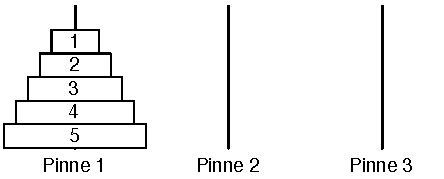
\includegraphics[scale=0.9]{img/hanoi-init.pdf}
\end{center}
De $n$ brickorna ska flyttas så att de hamnar i \Emph{avtagande} storlek på en av de övriga pinnarna. Detta ska ske i en följd av drag där man i varje drag flyttar den \Emph{översta} brickan från en pinne till en annan pinne. \Emph{Den bricka som flyttas får \Alert{aldrig} placeras ovanpå en \Alert{mindre} bricka.}
\end{Slide} 

\begin{Slide}{Krav}
\Emph{Krav}: Skriv ett program som börjar med att läsa in antalet brickor som ska flyttas. Därefter ska brickorna flyttas enligt reglerna. \\ \vspace{1em}Utskrift (exempel med tre brickor):
\begin{Code}
Flytta bricka 1 från pinne 1 till pinne 2
Flytta bricka 2 från pinne 1 till pinne 3
Flytta bricka 1 från pinne 2 till pinne 3
Flytta bricka 3 från pinne 1 till pinne 2
Flytta bricka 1 från pinne 3 till pinne 1
Flytta bricka 2 från pinne 3 till pinne 2
Flytta bricka 1 från pinne 1 till pinne 2
\end{Code}
\end{Slide} 

\begin{Slide}{Lösningsidé}
Det visar sig att \href{https://sv.wikipedia.org/wiki/Tornen_i_Hanoi}{Tornen i Hanoi} kan lösas med \href{https://en.wikipedia.org/wiki/Tower\_of\_Hanoi\#Non-recursive_solution}{denna strategi}:
\begin{itemize}
 \item I \Emph{udda} drag; drag nr 1, 3, \ldots\  flyttar man den minsta brickan, bricka 1, till pinnen närmast till höger. \\ Pinnen längst till vänster anses finnas ''till höger om'' pinnen längst till höger.
 \item I \Emph{jämna} drag; drag nr 2, 4, \ldots\  flyttar man en bricka mellan de två pinnar som inte innehåller bricka 1.
\end{itemize}
\pause
\vspace{2em}
Man kan bevisa att minsta antalet drag $N$ med $n$ brickor är: 
\begin{equation*}
N = 2^n - 1
\end{equation*}
\pause
Det finns många \href{https://www.youtube.com/watch?v=w9LgLiW9YHU}{filmer} på \href{https://www.youtube.com/watch?v=UMPneeBzQHk}{nätet} som \href{https://www.youtube.com/watch?v=h8JPtWpctl4}{visar} hur \href{https://www.youtube.com/watch?v=xUiDT3CjA40}{lösningen} går till.
\end{Slide} 

\begin{Slide}{Udda drag: flytta minstingen åt höger ''cirkulärt''} \footnotesize
Udda drag: Minstingen på pinne \code{i} flyttas till pinne \code{(i + 1) % 3}
\begin{center}
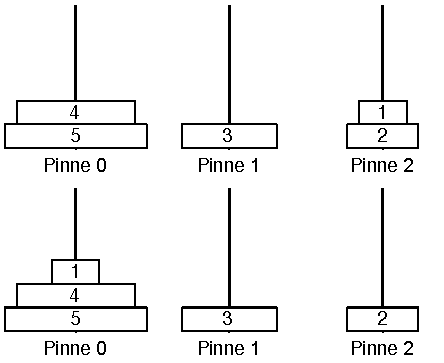
\includegraphics[scale=0.9]{img/hanoi-moves.pdf}
\end{center}
\end{Slide} 

\begin{Slide}{Design: Klasser och operationer}
\begin{center}
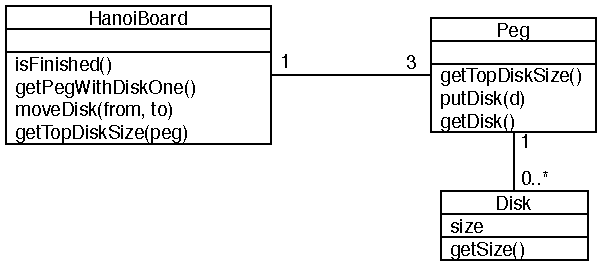
\includegraphics[scale=0.9]{img/hanoi-design.pdf}
\end{center}
\end{Slide} 

\begin{Slide}{Towers of Hanoi: huvudprogrammet}
\begin{Code}
import java.util.Scanner;

public class TowersOfHanoi {
    public static void main(String[] args) {
        System.out.print("Antal brickor: ");
        Scanner scan = new Scanner(System.in);
        int nbrDisks = scan.nextInt();
        scan.close();
        
        HanoiBoard board = new HanoiBoard(nbrDisks);
        HanoiStrategy strategy = new HanoiStrategy(board);
        strategy.moveDisks();
    }
}
\end{Code}
\end{Slide} 

\begin{Slide}{Specifikationer Disk och Peg}
\Emph{Övning}: Implementera \code{Disk} och \code{Peg} enligt specifikationerna.
\begin{ClassSpec}{Disk}
/** Skapar en bricka med storleken size */
public Disk(int size);

/** Tar reda på brickans storlek */
public int getSize();
\end{ClassSpec}
\begin{ClassSpec}{Peg}
/** Skapar en tom pinne */
public Peg();

/** Tar reda på numret på den översta brickan, Integer.MAX_VALUE om pinnen är tom */
public int getTopDiskSize();

/** Lägger brickan d överst på pinnen */
public void putDisk(Disk d);

/** Hämtar och tar bort den översta brickan */
public Disk getDisk();
\end{ClassSpec}
\end{Slide} 


\begin{Slide}{Specifikation HanoiBoard }
\begin{ClassSpec}{HanoiBoard}
/** Skapar en spelplan med tre tomma pinnar, lägger nbrDisks brickor på den
 *  första pinnen
 */
public HanoiBoard(int nbrDisks);

/** Tar reda på numret på pinnen som innehåller bricka 1 */
public int getPegWithDiskOne(); 

/** Undersöker om spelet är slut dvs om alla brickorna ligger på en annan
 *  pinne än den första
 */
public boolean isFinished();  

/** Tar reda på storleken av den översta brickan på pinne nummer peg,
 *  Integer.MAX_VALUE om pinnen är tom
 */
public int getTopDiskSize(int peg);

/** Flyttar den översta brickan från pinne nummer from till pinne nummer to
 */
public void moveDisk(int from, int to);   
\end{ClassSpec}
\Emph{Övning}: Implementera \code{HanoiBoard} enligt specifikationen.
\end{Slide} 

\begin{Slide}{Specifikation HanoiStrategy }
\begin{ClassSpec}{HanoiStrategy}
/**
 * Skapar en strategi för att flytta brickor på spelplanen board
 */
public HanoiStrategy(HanoiBoard board);

/**
 * Flyttar brickorna på pinne 1 till en annan pinne
 */
public void moveDisks() ;

/**
 * Flyttar en bricka enligt reglerna i drag nummer moveNbr, skriver ut
 * flyttningen
 */
private void moveOneDisk(int moveNbr);
\end{ClassSpec}
\Emph{Övning}: Implementera \code{HanoiStrategy} enligt specifikationen. \\ Ledning: se pseudo-kod på nästa bild.
\end{Slide} 

\begin{Slide}{Lösning, pseudo-kod}
\code{public void moveDisks()}
\begin{itemize}
\item \code{moveNbr = 1}
\item så länge spelet inte är slut
\begin{itemize}
\item \code{moveOneDisk(moveNbr)}
\item \code{moveNbr++}
\end{itemize}
\end{itemize}

\code{private void moveOneDisk(int moveNbr) }
\begin{itemize}
\item om \code{moveNbr} är udda:
\begin{itemize}
	 \item tag reda på numret på pinnen där bricka 1 finns
	 \item flytta den översta brickan från denna pinne till
	  pinnen närmast till höger modulo 3
\end{itemize}
\item annars:
\begin{itemize}
	 \item tag reda på numret på pinnen där bricka 1 finns
	 \item räkna ut numren på de båda andra pinnarna
	 \item flytta den minsta brickan mellan dessa pinnar
\end{itemize}
\end{itemize}
\end{Slide} 


\begin{Slide}{Lösning, implementation}
Se hela lösningen här:
\url{https://github.com/bjornregnell/lth-eda016-2015/tree/master/lectures/examples/eclipse-ws/lecture-examples/src/week13/hanoi}
\end{Slide} 
\Subsection{Inbjuden gäst: Patrik Persson lajvkodar androidapp}
\begin{Slide}{Designexempel: Skriv en app för Andorid}
\begin{itemize}
\item Med de kunskaper ni tillgodogör er i denna kurs är det hyffsat lätt att komma i gång med utveckling av mobilappar i den integrerade utvecklingsmiljön \href{https://en.wikipedia.org/wiki/Android_Studio}{Android Studio}.
\item Läs mer \href{http://techworld.idg.se/2.2524/1.602344/premiar-for-android-studio}{på techworld} och \href{http://developer.android.com/develop/index.html}{på officiella hemsidan}.
\item Inbjuden gästföreläsare Patrik Persson lajvkodar androidapp i Android Studio...
\end{itemize}
\begin{center}

\includegraphics[width=0.6\textwidth]{img/android-studio}
\end{center}
\end{Slide}


\end{document}	